%!TEX root = ../dokumentation.tex

\chapter{Python Code zur Steuerung des Systems}\label{chap:code}
Die gewählte Sprache, in welcher die Steuerung realisiert ist, ist Python. Python wurde gewählt, da mittels dieser die \acp{GPIO} des Raspberry Pi sehr einfach mittels einer Bibliothek ansteuerbar sind. Zudem ist Python eine sehr schnelle und weit verbreitete, hochentwickelte Programmiersprache.\\
Bei der Erstellung des Codes, welcher das System steuert, wurde von Anfang an eine objektorientierte Vorgehensweise gewählt. Dadurch wird eine möglichst reibungslose und fortschrittliche Umsetzung realisiert.\\
Der gesamte Code wird auf drei Dateien aufgeteilt. Dies dient zum einen zur besseren Übersichtlichkeit, zum anderen erhält jede Klasse eine eigene Datei.
\section{Motor}
Die erste Datei und Klasse beschäftigt sich mit der Ansteuerung der Schrittmotoren.\\
Sie benötigt zwei extra Bibliotheken (Listing \ref{motor_bib}). Die 'time' Bibliothek wird benötigt, um zwischen verschiedenen Befehlen 'schlafen' zu können, sprich das Programm pausieren zu können. Die 'RPI.GPIO' Bibliothek wird benötigt, um die \acp{GPIO} des Raspberry PI ansteuern zu können. 
\begin{lstlisting}[caption={Bibliotheken der Motor Klasse}, language={Python}, label={motor_bib}, numbers=left]
import time
import RPi.GPIO as GPIO	
\end{lstlisting}

\subsection{Konstruktor} 
Der Konstruktor der Klasse beschäftigt sich mit der Deklaration von Variablen und dem Zuweisen der dem Konstruktor übergebenen Parameter.\\
Im Falle der Motor Klasse bekommt der Konstruktor sechs Übergabeparameter, wovon allerdings ein Parameter ('self') eine Referenz auf das eigene Objekt ist.\\
Die restlichen übergebenen Parameter sind die \acp{GPIO}, welche für die Ansteuerung des Motortreibers benötigt werden.\\
Bei einem Blick auf den Code des Konstruktors (Listing \ref{motor_contructor}), sieht man die Übernahme der Übergabeparameter in klasseneigene Variablen (Zeile 2-6). Anschließend wird die Kommunikationsrichtung der \acp{GPIO} festgelegt (Zeile 7 - 11). In diesem Fall werden alle Pins als Ausgang benötigt.\\
Außerdem wird den \acp{GPIO} direkt ein Zustand zugewiesen (Zeile 12 - 16), in diesem Fall ist die Konfiguration so, dass der Motortreiber mit Achtelschritten arbeitet und den Motor gegen den Uhrzeigersinn drehen lässt.
\begin{lstlisting}[caption={Konstruktor der Motor Klasse}, language={Python}, label={motor_contructor}, numbers=left]
def __init__(self, Step, Dir, MS1, MS2, MS3):
    self.step = Step
    self.dir = Dir
    self.MS1 = MS1
    self.MS2 = MS2
    self.MS3 = MS3
    GPIO.setup(self.step, GPIO.OUT)
    GPIO.setup(self.dir, GPIO.OUT)
    GPIO.setup(self.MS1, GPIO.OUT)
    GPIO.setup(self.MS2, GPIO.OUT)
    GPIO.setup(self.MS3, GPIO.OUT)
    GPIO.output(self.step, GPIO.LOW)
    GPIO.output(self.dir, GPIO.LOW)
    GPIO.output(self.MS1, GPIO.HIGH)
    GPIO.output(self.MS2, GPIO.HIGH)
    GPIO.output(self.MS3, GPIO.LOW)
\end{lstlisting}
\subsection{Bewegen des Motors}
Die Motor Klasse besitzt zudem noch eine Funktion, mittels welcher sich der jeweilige Motor bewegen lässt (Listing \ref{motor_move}). In der Funktion wird zunächst die Drehrichtung je nach Übergabeparameter gesetzt (Zeile 2 - 5). Anschließend wird ein bzw. je nachdem wie viele Schritte gefordert werden, ausführt. Um einen kompletten Schritt zu vollenden, wird der dafür vorgesehene Pin des Motortreibers Ein und wieder Aus geschaltet. Die Zeit zwischen diesen beiden Vorgängen kann über einen Übergabeparameter der Funktion eingestellt werden (Zeile 8 - 13). Dies bestimmt direkt die Drehgeschwindigkeit des Motors. Wird eine geringe Zeit übergeben, wird eine schnellere Drehung des Motors erreicht. 
\begin{lstlisting}[caption={Funktion zum Bewegen des Motors}, language={Python}, label={motor_move}, numbers=left]
def moveMotor(self, dir, step, speed):
    if(dir):
        GPIO.output(self.dir, GPIO.HIGH)
    else:
        GPIO.output(self.dir, GPIO.LOW)

    i = 0
    while i < step:
        GPIO.output(self.step, GPIO.HIGH)
        time.sleep(speed)
        GPIO.output(self.step, GPIO.LOW)
        time.sleep(speed)
        i += 1
\end{lstlisting}


\section{Lidar}
Auch der \ac{LIDAR} Sensor hat eine eigene Datei sowie Klasse. Dies soll dazu dienen, mehrere verschiedene Sensoren konfigurieren zu können und diese dann schnell und einfach mit denselben Funktionen auswählen zu können.\\
Die Klasse ist in ihrer jetzigen Form bereits in der Lage zwei verschiedene \ac{LIDAR} Sensoren zu bedienen.
Die Lidar Klasse benötigt zwei Bibliotheken (Listing \ref{lidar_bib}). Mit der ersten kann eine serielle Verbindung erstellt werden. Die zweite Bibliothek wird benötigt, um einen der zwei Möglichen \ac{LIDAR} Sensoren anzusteuern. 
\begin{lstlisting}[caption={Bibliotheken der Lidar Klasse}, language={Python}, label={lidar_bib}, numbers=left]
import serial
import VL53L1X
\end{lstlisting}

\subsection{Konstruktor und Variablen}
Die Lidar Klasse besitzt zwei Variablen. Die Variable 'dist' wird verwendet, um die gemessene Entfernung zu speichern und auf diese zugreifen zu können.\\
Die zweite Variable wird als Flag bei Verwendung des \ac{LIDAR} Sensors 'TFMini' (Kapitel \ref{tf_mini}) benötigt (Listing \ref{lidar_constructor}).\\
Der Konstruktor der Klasse ist zudem in der Lage, je nachdem welche Parameter angegeben werden, die korrekte Verbindung herzustellen. Je nachdem welche Werte angegeben und welche als "None"  definiert werden, stellt der Konstruktor entweder eine Verbindung über \ac{UART} (Zeile 9) oder \ac{I$^{2}$C} (Zeile 11 - 13) her. 
\begin{lstlisting}[caption={Kostruktor der Lidar Klasse}, language={Python}, label={lidar_constructor}, numbers=left]
class LIDAR():
    dist = 0
    recievedData = False

    def __init__(self, uart, i2c):
        self.uart = uart
        self.i2c = i2c
        if(self.uart != None and self.i2c == None):
            self.ser = serial.Serial(self.uart, 115200, timeout=1)
        else:
            self.tof = VL53L1X.VL53L1X(i2c_bus=1, i2c_address=i2c)
            self.tof.open()
            self.tof.start_ranging(3)
\end{lstlisting}
\subsection{Aufnehmen von Messdaten}
Die Funktion um Daten vom \ac{LIDAR} Sensor zu bekommen ist auch in der Klasse definiert. Somit kann für egal welchen Sensortyp über die selben Funktionsaufrufe die Distanz ermittelt werden. 
\begin{lstlisting}[caption={Funktion um Distanz vom \ac{LIDAR} Sensor zu erhalten}, language={Python}, label={lidar_getData}, numbers=left]
	def getData(self):
        if(self.uart != None and self.i2c == None):
            self.ser.reset_input_buffer()
            while(self.recievedData != True):
                while(self.ser.in_waiting <= 9):
                    if((b'Y' == self.ser.read()) and (b'Y' == self.ser.read())):
                        Dist_L = self.ser.read()
                        Dist_H = self.ser.read()
                        self.dist = (ord(Dist_H) * 256) + (ord(Dist_L))
                        for i in range (0,5):
                            self.ser.read()
                        self.recievedData = True
                        break
        else:
            self.dist = self.tof.get_distance() # Entfernung in mm
            self.dist = self.dist/10.0
\end{lstlisting}
In Listing \ref{lidar_getData} kann man sehen, dass ähnlich wie im Konstruktor je nachdem welcher Sensor 'ausgewählt' wurde, unterschiedliche Methoden verwendet werden um Daten zu bekommen. Der erste Abschnitt in Zeile 3 - 13 ist für die Verwendung eines Sensors mittels \ac{UART} gedacht. Da \ac{UART} ein serieller Bus ist, auf welchen vom Slave konstant Daten geschickt werden, wartet diese Funktion so lange, bis neue Daten ankommen. Die neuen Daten werden durch zwei aufeinanderfolgende 'Y' gekennzeichnet. Anschließend werden die zwei Byte für die Entfernung gespeichert (Zeile 7 \& 8) und zur Gesamtdistanz zusammengefügt (Zeile 9). Anschließend wird die bereits erwähnte Flag der Klasse gesetzt, damit nur ein einzelner Wert aufgenommen wird.\\
Die zweite Methode in Zeile 15 - 16 ist deutlich einfacher, da hierbei eine Bibliothek verwendet werden kann. Dabei muss die Distanz lediglich in die richtige Größe konvertiert werden (Zeile 15 - 16).
\newpage
\section{Steuerung}
Die dritte und letzte Datei beschäftigt sich mit der generellen Steuerung des Systems und dem Initialisieren und Aufrufen der Klassen und derer Funktionen.\\
Für die Steuerung des Systems werden einige Bibliotheken mehr benötigt.
\begin{lstlisting}[caption={Bibliotheken zur Steuerung des Systems}, language={Python}, label={main_bibliotheken}, numbers=left]
# Bibliotheken
import time
import datetime
import math
import RPi.GPIO as GPIO

# Eigene Dateien
import Lidar
import Motor

# GPIO Nummerierung gleich der Pin Nummer
GPIO.setmode(GPIO.BOARD)
GPIO.setwarnings(False)
\end{lstlisting}
Die Bibliotheken in Zeile 2 \& 3 (Listing \ref{main_bibliotheken})werden für die Benennung der Dateien, welche produziert werden, benötigt. Die 'math' Bibliothek wird für einige Berechnungen verwendet und die 'RPi.GPIO' wird wie bereits erwähnt benötigt, um die \acp{GPIO} des Raspberry Pi möglichst einfach anzusteuern. Anschließend werden dann noch die zwei Klassen importiert, welche in den vorangegangenen Abschnitten erklärt werden. Zudem wird noch der Modus der \ac{GPIO} Nummerierung festgelegt. In diesem Fall ist der Modus gleich der Nummerierung der Pins auf dem Board. 
\begin{figure}[H]
	\centering
	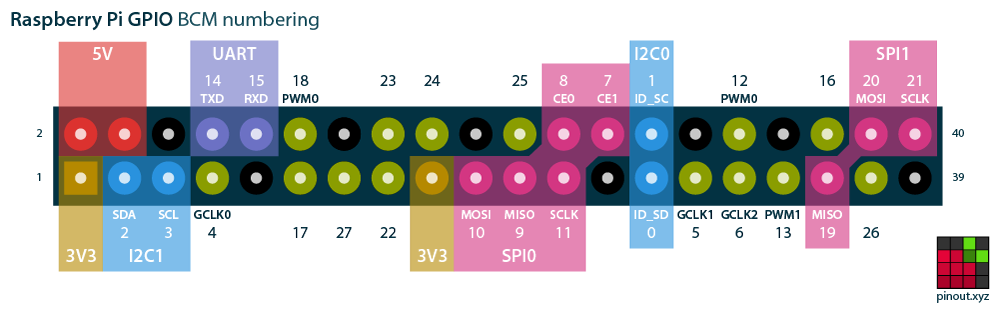
\includegraphics[width=0.75\textwidth]{images/Code/raspberry-pi-pinout}
	\caption{Raspberry Pi pinout \cite{raspi_pinout}}
	\label{raspi_pinout}
\end{figure}
\subsection{Pin Definitionen und Initialisieren der Klassen}
Da wie in den vorangegangenen Kapiteln erläutert Klassen für Motor und Lidar erstellt wurden, müssen diese nun aufgerufen und initialisiert werden. Zudem sind weitere \acp{GPIO} nötig um das gesamte System zu Steuern.
\begin{lstlisting}[caption={Initialisieren von Variablen und Klassen}, language={Python}, label={main_classes}, numbers=left]
# Pins & Definitionen
workingLED = 11
fan = 13
lightGate = 23 #SPI SCLK --> In Version 2 der Platine eigenen Pin zuweisen

# Motor 1, Nema 11
M1 = Motor.MOTOR(31,29,37,35,33)

# Motor 2, Nema 17
M2 = Motor.MOTOR(18,16,36,38,40)

# LIDAR Sensor
lidar = Lidar.LIDAR('/dev/ttyAMA0', none)
#lidar = Lidar.LIDAR(None, 0x29)
\end{lstlisting}
Zunächst werden die Pins für die verschiedenen, auf der Platine vorgesehenen, Funktionen definiert (Listing \ref{main_classes}). Eine Anmerkung hierzu ist, dass auf der Platine versäumt wurde einen Pin für die Lichtschranke zur Positionierung bereitzustellen. Daher wird hier der Pin verwendet, welcher eigentlich für den seriellen Takt des \ac{SPI} zuständig ist. Außerdem werden Pins für eine Status \ac{LED} und einen Lüfter bereitgestellt. \\
Nach den normalen Pin Deklarationen werden die beiden Motoren durch die Klassen initialisiert. Dazu werden, wie im Kapitel der Motorklasse beschrieben, die verschiedenen Pins zur Ansteuerung des Motortreibers dem Konstruktor der Klasse übergeben. Anschließend kann der Motor mittels den in der Klasse definierten Funktionen gesteuert werden.\\
Zuletzt muss nur noch der \ac{LIDAR} Sensor initialisiert werden. Dazu kann wie in Zeile 13 \& 14 zu sehen ist, eine der beiden Initialisierungsmöglichkeiten gewählt werden, um entweder einen Sensor mittels \ac{UART} oder \ac{I$^{2}$C} zu verwenden.\\
\subsection{Zusätzliche Funktionen}
Nachdem alle benötigten Variablen für die \acp{GPIO} definiert sind, werden noch einige Funktionen benötigt, um einen schöneren und übersichtlicheren Code zu erzeugen (Listing \ref{main_functions}). 
\begin{lstlisting}[caption={Funktionen für die Übersichtlichkeit des Codes}, language={Python}, label={main_functions}, numbers=left]
# Funktion um GPIO's zu Initalisieren
def initGPIO():
    GPIO.setup(workingLED, GPIO.OUT)
    GPIO.output(workingLED, GPIO.LOW)
    GPIO.setup(fan, GPIO.OUT)
    GPIO.output(fan, GPIO.LOW)
    GPIO.setup(lightGate, GPIO.IN)

def homeAxis():
    while(GPIO.input(lightGate)!=GPIO.HIGH):
        M2.moveMotor(1,1,0.001)
    count = 0
    while(GPIO.input(lightGate)==GPIO.HIGH):
        M2.moveMotor(1,1,0.001)
        count += 1
    M2.moveMotor(1,36,0.001)
\end{lstlisting}
Die erste Funktion (Zeile 2 - 7) dient dazu, die übrigen \acp{GPIO} zu initialisieren und diesen einen Startwert zu geben. Hier werden die \acp{GPIO}, welche für die LED und den Lüfter vorgesehen sind als Ausgang deklariert und als 'LOW' initialisiert. Der \ac{GPIO} Pin, welcher für die Lichtschranke vorgesehen ist, wird als Eingang deklariert.\\
Die zweite Funktion wird benötigt, um das System in horizontaler Richtung in die Ausgangslage zu bringen. Dazu wird der Motor 2, welcher für den Azimutwinkel zuständig ist, so lange gedreht, bis dieser die Lichtschranke erreicht und diese wieder verlässt. Da die Lichtschranke nicht zu 100\% am Kreisscheitelpunkt positioniert ist, wird nach verlassen der Lichtschranke mit einem manuellen Kalibrationswert (Zeile 16) der Azimutwinkel in Nulllage gebracht.\\
\subsection{Variablendeklaration und Aufrufen von Funktionen}
Bevor mit dem eigentlichen Messen begonnen werden kann, müssen noch einige Variablen definiert und Funktionen aufgerufen werden.
\begin{lstlisting}[caption={Aufrufen von Funktionen und Variablen deklaration}, language={Python}, label={main_setup}, numbers=left]
initGPIO()
lidar.getData()
lidar.recievedData = False
homeAxis()
time.sleep(2)

stepsFullRotM2 = 200*8*6
stepsQuartRotM1 = 50*4

M1dir = False
M2dir = True

lidar.getData()
print(lidar.dist)
lidar.recievedData = False

data = open("data_"+datetime.datetime.fromtimestamp(time.time()).strftime('%Y-%m-%d_%H-%M-%S')+".csv", "w")
data.write("Nr;Distance;Azimut;Elevation\n")
valueNr = 1
\end{lstlisting}
In Zeile 1 (Listing \ref{main_setup}) werden zuerst die \acp{GPIO} initialisiert. Anschließend wird ein Wert vom \ac{LIDAR} ausgelesen  und die Flag des \acp{LIDAR} wieder auf 'False' gesetzt, damit dieser anschließend wieder Messwerte aufnehmen kann. Dies dient zum Funktionstest, bevor das System bewegt wird. Wenn der Sensor beispielsweise nicht korrekt verbunden wird, würde das System abbrechen, bevor etwas bewegt wird. Danach wird das System in die Ausgangslage positioniert und eine kurze Zeit gewartet, bevor es mit dem eigentlichen Messvorgang losgeht.\\
Wie in Zeile 7 \& 8 zu sehen, werden anschließend noch die Anzahl der benötigten Schritte für eine ganze Umdrehung und eine Viertelumdrehung berechnet. Diese Werte werden benötigt, um die Grenzen für die Schleifen der Messung festzulegen. Ein Schrittmotor macht pro Umdrehung 200 ganze Schritte. Da eine hohe Auflösung gewünscht ist, wird die Mikroschrittfunktion der Motortreiber verwendet. Im Fall der verwendeten Motortreiber werden Achtelschritte gewählt. Allerdings hat der Motortreiber 1, welcher für die vertikale Achse zuständig ist einen Fehler, wodurch nur viertel Schritte möglich sind.\\
In Zeile 10 \& 11 werden die Startrichtungen für die Motoren festgelegt.\\
Anschließend wird ein Messwert in die Konsole ausgegeben, um dem Bediener eine Rückmeldung zu geben, dass das System ordnungsgemäß funktioniert.\\
\subsection{Erstellen der Datei zum Speichern der Daten}
Ein letzter Schritt ist noch notwendig bevor mit der Messung begonnen werden kann (Listing \ref{main_data}). Dabei wird die Datei, in welcher die Messwerte abgespeichert werden, erstellt. Die Datei wird dabei immer mit 'data' und dem aktuellen Datum sowie Timestamp versehen. Als letzte Aktion vor der Messung wird der Index des ersten Messwertes gleich 1 gesetzt.\\
\begin{lstlisting}[caption={Erstellen der Datei zum Speichern der Daten}, language={Python}, label={main_data}, numbers=left]
data = open("data_"+datetime.datetime.fromtimestamp(time.time()).strftime('%Y-%m-%d_%H-%M-%S')+".csv", "w")
data.write("Nr;Distance;Azimut;Elevation\n")
valueNr = 1
\end{lstlisting}
Die \ac{csv} Datei, in welcher die Daten gespeichert werden, ist nach folgendem Schema aufgebaut:
\begin{table}[H]
	\centering
	\caption{Beispieldatei}
	\begin{tabular}{|l|l|l|l|}
		\hline
		\textbf{Nr} & \textbf{Distance} & \textbf{Azimut} & \textbf{Elevation} \\\hline
		1  & 105      & 0       & 0         \\\hline
		2  & 105      & 0.18       & 0      \\\hline
		3  & 106      & 0.36       & 0      \\\hline
	\end{tabular}
\end{table}
Jeder Wert, welcher in die Datei gespeichert wird, bekommt einen Index. Somit kann man einen Überblick behalten, wie viele Messwerte aufgezeichnet wurden. Die zweite Spalte, welche in der Datei steht, ist für die Distanz vorgesehen, welche vom \ac{LIDAR} Sensor ermittelt wird. Die beiden letzten Spalten dienen der Speicherung des Winkels, welcher aus der Position der Schrittmotoren ermittelt wird. Die Distanz wird in $cm$ gespeichert und die beiden Winkel in Grad.

\subsection{Schleifen der Steuerung}
\begin{lstlisting}[caption={Messen und Aufzeichnen der Entfernungen}, language={Python}, label={main_loop}, numbers=left]
countM1 = 0
countM2 = 0
while(countM1 < stepsQuartRotM1):
    if(M2dir):
        while(countM2 < stepsFullRotM2):
            lidar.getData()
            lidar.recievedData = False
            data.write(str(valueNr) + ";" + str(lidar.dist) + ";" + str(360.0*countM2/stepsFullRotM2) + ";" + str(90.0*countM1/stepsQuartRotM1) + "\n")
            M2.moveMotor(M2dir,4,0.00025)
            valueNr += 1
            countM2 += 4
    else:
        while(countM2 >= 0):
            lidar.getData()
            lidar.recievedData = False
            data.write(str(valueNr) + ";" + str(lidar.dist) + ";" + str(360.0*countM2/stepsFullRotM2) + ";" + str(90.0*countM1/stepsQuartRotM1) + "\n")
            M2.moveMotor(M2dir,4,0.00025)
            valueNr += 1
            countM2 -= 4
    M1.moveMotor(M1dir,4,0.0005)
    countM1 += 4
    M2dir = not M2dir

data.stop()
lidar.tof.stop_ranging()
\end{lstlisting}
Da in Python keine konventionellen 'for' Schleifen möglich sind, müssen 'while' Schleifen verwendet werden. Dazu wird eine extra Variable benötigt (Zeile 1 \& 2 Listing \ref{main_loop}) um zu überwachen, wie oft die Schleife schon durchlaufen wurde. Da in diesem Fall zwei 'while' Schleifen ineinander verschachtelt wurden, werden auch zwei Variablen benötigt um die Anzahl der Durchläufe zu überwachen. \\
Die äußere Schleife wird nur so oft durchlaufen, bis der Motor 1, welcher für die Neigung des Polarwinkles (Elevation) zuständig ist, 90° erreicht. Im inneren dieser Schleife gibt es eine Besonderheit. Da sich die Kabel des oberen Aufbaus nur endlich oft drehen können bis diese verschleißen, muss das System nach jeden 360° die Richtung umkehren. Dafür werden 2 verschiedene Schleifen benötigt, da später der Winkel anhand des Counters der Schleifendurchläufe berechnet wird. Prinzipiell passiert in den Schleifen in Zeile 5 - 11 und Zeile 13 - 19 aber exakt das selbe. Zuerst werden neue Daten vom \ac{LIDAR} Sensor angefragt, und die Flag des Sensors gesetzt. Anschließend wird der ermittelte Wert zusammen mit den aktuellen Winkeln und einem Index in die '.csv' Datei gespeichert. Die Winkel werden dabei in Grad angegeben (Zeile 8 \& 16).\\
Nachdem die Werte gespeichert wurden, wird der Motor bewegt. In diesem Fall um vier Schritte. Dies zeigt, dass das System in diesem Codebeispiel nur mit einem Viertel der Auflösung in horizontaler Richtung arbeitet. Anschließend wird der Index sowie der Schleifenzähler erhöht. Beim Schleifenzähler besteht der große Unterschied zwischen den beiden 'while' Schleifen, da einmal die Schleife von 'vorne' und einmal von 'hinten' durchlaufen wird. Die Schrittweite Vier ergibt sich aus der Anzahl der Schritte welche auch dem Motor übergeben wurden.\\
Wenn die innere Schleife eine volle 360° Drehung, also eine komplette Rotation durchlaufen hat, wird der Motor 1, welcher für den Polarwinkel zuständig ist ebenfalls bewegt. In diesem Fall auch um vier Schritte was ein Viertel der vertikalen Auflösung bedeutet. Der zweite Schleifenzähler wird ebenfalls um Vier erhöht, und die Richtung des Motors für die horizontale Drehung wird umgekehrt, bevor die innere Schleife aufs neue durchlaufen wird.\\
Wenn die gesamte Messung abgeschlossen ist, wird die Datei, welche die Daten enthält geschlossen und die Messung gestoppt. Die Datei kann nun weiterverwendet und ausgewertet werden.
